% Manuscript insertion fragment; requires amsmath, amssymb, and graphicx.
% The figure path is relative to the repository root.
% All four panels are arranged in one horizontal row.

\paragraph{Sensitivity to partition resolution.}
We study partition sensitivity through entropy RMSE, illustrating the tradeoff
between approximation and estimation errors suggested by the bound.
In Fig.~\ref{fig:ell-comparison}, the two left panels (a,b) use the density
\[
f_d(\mathbf{x})=1+0.7\cos\!\bigl(2\pi(x_1-x_2)\bigr),
\qquad \mathbf{x}\in[0,1]^d.
\]
It has uniform marginals and satisfies $0.3\le f_d\le1.7$, with Lipschitz
constant $1.4\pi\sqrt{2}$ on the cube, independently of $d$.
The two right panels (c,d) use centered equicorrelated Gaussian data with
unit marginal variances and $\rho=0.2$, exploring the rule beyond the
theorem's compact-support and positive-lower-bound assumptions.

Panels (a,c) fix $n=10^5$ and vary $d\in\{2,3,4\}$.
Panel (b) fixes $d=2$ and varies $n\in\{10^3,10^4,10^5\}$;
panel (d) fixes $d=3$ and varies $n\in\{3\times10^4,10^5,3\times10^5\}$.
The bounded and Gaussian settings use 100 and 30 independent repetitions,
respectively, with grids $\mathcal{L}=\{1,\ldots,7\}$ and
$\mathcal{L}=\{1,\ldots,8\}$.
We compare empirical RMSE minima with the \emph{theory-selected} resolution
\begin{equation}
\begin{aligned}
\ell_{\mathrm{th}}
&=\underset{\ell\in\mathcal{L}}{\operatorname{arg\,min}}
\left\{\ell^{-2}+\sqrt{\Lambda_{n,d,\delta}}
\left(\frac{\ell^d}{n}\right)^{1/4}\right\},\\
\Lambda_{n,d,\delta}
&=2d\log(2n+1)+\log(96/\delta),\qquad\delta=0.05.
\end{aligned}
\label{eq:ell-comparison-selection}
\end{equation}
The bound's common positive factor $Kd$ cancels; no coefficient is fitted.
These are exploratory examples: the bounded panels retain five of seven
evaluated settings, and the Gaussian panels follow a correlation sweep.
The choices agree in three of five bounded and four of five Gaussian settings.
Empirical minima use the same repetitions as the curves and do not establish
finite-sample RMSE optimality.

\begin{figure*}[t]
\centering
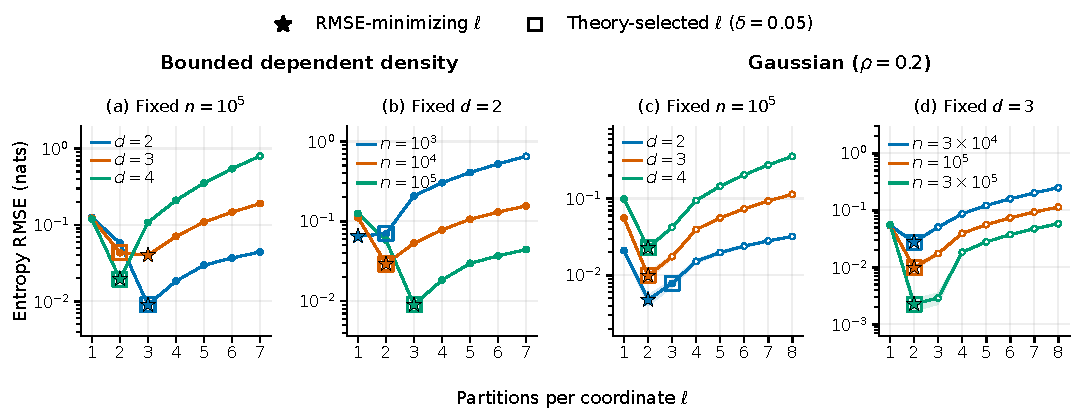
\includegraphics[width=\textwidth]{experiments/synthetic_ell_comparison/figures/bounded_gaussian_ell_rmse.pdf}
\caption{Entropy RMSE versus partitions per coordinate $\ell$.
Panels (a,b) use the bounded dependent density; panels (c,d) use Gaussian
data with $\rho=0.2$.
Panels (a,c) vary dimension at $n=10^5$; panels (b,d) vary sample size at
$d=2$ and $d=3$, respectively.
Results use 100 bounded or 30 Gaussian repetitions.
Shading shows pointwise 95\% bootstrap intervals from 2,000 resamples.
Stars indicate empirical grid minima without a coverage filter; squares
indicate the theory-selected resolution.
Open circles indicate incomplete coverage in at least one repetition.
Each distribution contributes five unique settings, with one shared setting
appearing in both corresponding panels.}
\label{fig:ell-comparison}
\end{figure*}
